There are a lot of applications and services that do real-time communications out on the market today. First we will take a look at similar technologies\cite{lopez_fernandez_catalysing_2013} that is in direct competition with \gls{wrtc}, in addition we will look at businesses that are looking to incorporate real-time communications in their existing services.

\subsection{Real-time communications}
For doing real-time communications the biggest vendors are Cisco, Polycom, and Microsoft as seen in figure \ref{fig:room-based-videoconferencing} and figure \ref{fig:desktop-videoconferencing}.

\begin{figure}[here]
\centerline{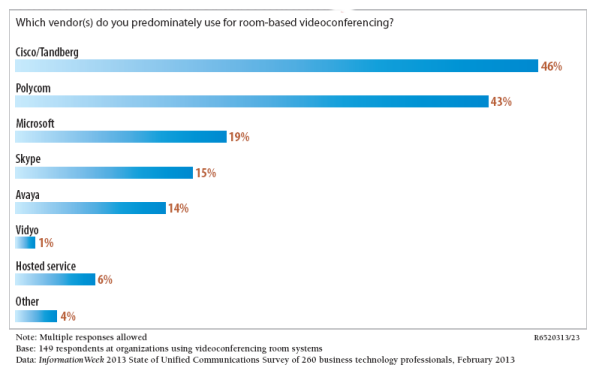
\includegraphics[scale=0.75]{room-based-videoconferencing.png}}
\label{fig:room-based-videoconferencing}
\caption{Vendors used for room-based videoconferencing}
\end{figure}

\begin{figure}[here]
\centerline{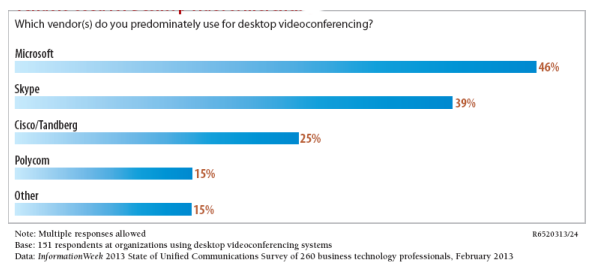
\includegraphics[scale=0.75]{desktop-videoconferencing.png}}
\caption{Vendors used for desktop videoconferencing}
\label{fig:desktop-videoconferencing}
\end{figure}

Cisco is clearly the big winner with their room-based videoconferencing systems, but Microsft is winning the desktop market with their Lync and Skype applications. Skype utilizes a peer-to-peer model by leveraging all of the available resources in a network, this is probably why they can manage free communications, as using centralized resources are very costly. Skype has very successfully developed an audio/video communications platform with their technology, however the same type of model is used by \gls{wrtc} to allow for efficient use of resources.

\subsection{Customer-service}
Customer-services depend heavily on communications, but these services have mostly been concentrated around the traditional telephone and more recently browser based chat messaging. Now there is a trend to incorporate live chat with video as well in this market\cite{amazon_mayday}. It's all about having a personal experience and engaging with the customer. Especially e-commerce sites are looking to integrate \gls{wrtc} as part of their customer service experience, and with \gls{wrtc} it is easy to add in video support as well.

\subsection*{Summary}
These companies have made significant investments to build their services, and with the introduction of \gls{wrtc} these companies are threatened by upcoming competing businesses. It's exciting to see where the market is going to shift, both Cisco and companies that use \gls{wrtc} has the advantage of being able to deliver platform independant applications, but Microsoft are still slow with delivering to any other platform than Windows.